\documentclass{beamer}
\usepackage{listings}
\usepackage{booktabs}
\usepackage{tikz}
\usepackage{verbatim}

\usetheme{Warsaw}
\title[Adventure]{Colossal Cave Adventure in Python\\ \dots in the browser!}
\author[@chris\_{}swenson]{Christopher Swenson}
\date[PyCon 2018]{PyCon; May 12, 2018}

\lstdefinelanguage{JavaScript}{
  keywords={typeof, new, true, false, catch, function, return, null, catch, switch, var, if, in, while, do, else, case, break},
  keywordstyle=\bfseries,
  ndkeywords={class, export, boolean, throw, implements, import, this},
  ndkeywordstyle=\color{darkgray}\bfseries,
  identifierstyle=\color{black},
  sensitive=false,
  comment=[l]{//},
  morecomment=[s]{/*}{*/},
  commentstyle=\color{purple}\ttfamily,
  stringstyle=\color{red}\ttfamily,
  morestring=[b]',
  morestring=[b]"
}

\lstloadlanguages{[77]Fortran,Python,JavaScript}

\def\py{
  \lstset{
     language=Python,
     %backgroundcolor=\color{lightgray},
     extendedchars=true,
     basicstyle=\footnotesize\ttfamily,
     showstringspaces=false,
     showspaces=false,
     %numbers=left,
     %numberstyle=\footnotesize,
     numbersep=9pt,
     tabsize=2,
     breaklines=true,
     showtabs=false,
     captionpos=b
  }
}

\def\fortran{
  \lstset{
     language=[77]FORTRAN,
     %backgroundcolor=\color{lightgray},
     keywordstyle=\bfseries,
     extendedchars=true,
     basicstyle=\footnotesize\ttfamily,
     showstringspaces=false,
     showspaces=false,
     %numbers=left,
     %numberstyle=\footnotesize,
     numbersep=9pt,
     tabsize=8,
     breaklines=true,
     showtabs=false,
     captionpos=b
  }
}

\def\js{
  \lstset{
     language=JavaScript,
     %backgroundcolor=\color{lightgray},
     extendedchars=true,
     basicstyle=\ttfamily,
     showstringspaces=false,
     showspaces=false,
     %numbers=left,
     %numberstyle=\footnotesize,
     numbersep=9pt,
     tabsize=2,
     breaklines=true,
     showtabs=false,
     captionpos=b
  }
}

\begin{document}

\begin{frame}
\titlepage
\end{frame}

\begin{frame}{What is this talk?}

What is this talk?

\ \\
Colossal Cave Adventure, the PDP-10, FORTRAN IV, and a Python interpreter written in JavaScript.

\ \\

Who is this talk for?

\ \\

Curious programmery people

\ \\

Slides available on GitHub:
\url{https://swenson.github.io/adventure-talk-pycon}

\end{frame}

\begin{frame}{Who am I?}


%\ \\

Christopher Swenson, Ph.D

\ \\

Currently at Twilio (prev.\ Google, Government, Simple)

\ \\

Occasional BeeWare core contributor and PyDX organizer

\ \\

I love programming languages and stuff.

\end{frame}

\begin{frame}{Motivation}
Idea: write a game with text messaging!

\ \\

\dots why not ``port'' the first text adventure?!

\end{frame}

\begin{frame}{ADVENTURE}

ADVENTURE

\ \\

a.k.a., Colossal Cave

\ \\

1976 text adventure, probably the first

\ \\

Wildly popular and influential

\ \\

Written in FORTRAN IV for the PDP-10 (defunct)

\ \\

Text to +1 (669) 238-3683 to play now!

\end{frame}

\begin{frame}[fragile]{ADVENTURE beginning}

\begin{verbatim}
SOMEWHERE NEARBY IS COLOSSAL CAVE, WHERE OTHERS HAVE FOUND
FORTUNES IN TREASURE AND GOLD, THOUGH IT IS RUMORED
THAT SOME WHO ENTER ARE NEVER SEEN AGAIN. MAGIC IS SAID
TO WORK IN THE CAVE. I WILL BE YOUR EYES AND HANDS. DIRECT
ME WITH COMMANDS OF 1 OR 2 WORDS.
(ERRORS, SUGGESTIONS, COMPLAINTS TO CROWTHER)
(IF STUCK TYPE HELP FOR SOME HINTS)

YOU ARE STANDING AT THE END OF A ROAD BEFORE A SMALL BRICK
BUILDING . AROUND YOU IS A FOREST. A SMALL
STREAM FLOWS OUT OF THE BUILDING AND DOWN A GULLY.
\end{verbatim}

\end{frame}

\begin{frame}{PDP-10}
Pic from \url{http://www.columbia.edu/cu/computinghistory/pdp10.html}

\begin{center}
  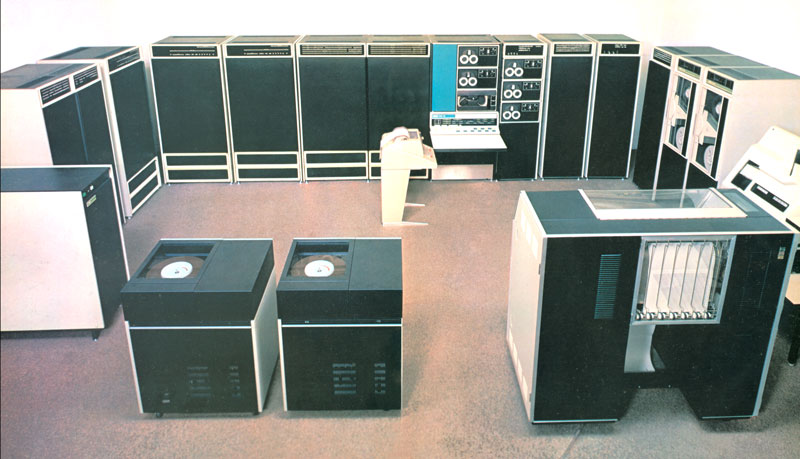
\includegraphics[width=.75\textwidth]{ka10.jpg}
\end{center}
\end{frame}
\begin{frame}{PDP-10 FORTRAN IV}
  We're talking all the good stuff:

\begin{itemize}
  \item All caps
  \item No recursion
  \item Line numbers
  \item Spaces don't matter
  \item Punch cards
\end{itemize}

\end{frame}
\begin{frame}[fragile]{Code}

\fortran
\begin{lstlisting}
C ADVENTURES
	IMPLICIT INTEGER(A-Z)
	REAL RAN
	COMMON RTEXT,LLINE
	DIMENSION IOBJ(300),ICHAIN(100),IPLACE(100)
	1 ,IFIXED(100),COND(300),PROP(100),ABB(300),LLINE(1000,22)
	2 ,LTEXT(300),STEXT(300),KEY(300),DEFAULT(300),TRAVEL(1000)
	3 ,TK(25),KTAB(1000),ATAB(1000),BTEXT(200),DSEEN(10)
	4 ,DLOC(10),ODLOC(10),DTRAV(20),RTEXT(100),JSPKT(100)
	5 ,IPLT(100),IFIXT(100)
\end{lstlisting}

\end{frame}

\begin{frame}[fragile]{Code (cont'd.)}

\fortran
\begin{lstlisting}
C READ THE PARAMETERS

	IF(SETUP.NE.0) GOTO 1
	SETUP=1
	KEYS=1
	LAMP=2
	GRATE=3
C ...
	DATA(JSPKT(I),I=1,16)/24,29,0,31,0,31,38,38,42,42,43,46,77,71
	1 ,73,75/
	DATA(IPLT(I),I=1,20)/3,3,8,10,11,14,13,9,15,18,19,17,27,28,29
	1 ,30,0,0,3,3/
\end{lstlisting}
\end{frame}

\begin{frame}[fragile]{Code (cont'd.)}
\fortran
\begin{lstlisting}
	DO 1001 I=1,300
	STEXT(I)=0
	IF(I.LE.200) BTEXT(I)=0
	IF(I.LE.100)RTEXT(I)=0
1001	LTEXT(I)=0
\end{lstlisting}
\end{frame}

\begin{frame}[fragile]{Code (cont'd.)}
\fortran
\begin{lstlisting}
1002	READ(1,1003) IKIND
1003	FORMAT(G)
\end{lstlisting}
\end{frame}

\begin{frame}[fragile]{Computed GOTO}
\fortran
\begin{lstlisting}
        GOTO(1100,1004,1004,1013,1020,1004,1004)(IKIND+1)
\end{lstlisting}
\end{frame}

\begin{frame}[fragile]{Reading data}
\fortran
\begin{lstlisting}
1004	READ(1,1005)JKIND,(LLINE(I,J),J=3,22)
1005	FORMAT(1G,20A5)
\end{lstlisting}
\end{frame}

\begin{frame}[fragile]{Calling subroutines}
\fortran
\begin{lstlisting}
1	CALL YES(65,1,0,YEA)
\end{lstlisting}
\end{frame}

\begin{frame}[fragile]{Subroutines}
\fortran
\begin{lstlisting}
	SUBROUTINE YES(X,Y,Z,YEA)
	IMPLICIT INTEGER(A-Z)
	CALL SPEAK(X)
	CALL GETIN(JUNK,IA1,JUNK,IB1)
	IF(IA1.EQ.'NO'.OR.IA1.EQ.'N') GOTO 1
	YEA=1
	IF(Y.NE.0) CALL SPEAK(Y)
	RETURN
1	YEA=0
	IF(Z.NE.0)CALL SPEAK(Z)
	RETURN
	END
\end{lstlisting}
\end{frame}

\begin{frame}{36-bit Words}
Pre-1980 or so, many different default word sizes

\ \\

Nowadays, 8/16/32/64/128/256 are common

\ \\
DEC (PDP, VAX) used 12, 36, 32
\end{frame}
\begin{frame}{36-bit ASCII???}
PDP-10 (1966) used 7-bit ASCII from 1963

\ \\

ASCII not quite what we know until 1967
\ \\

36/7 = 5 (with 1 bit remainder)\ \\
\end{frame}
\begin{frame}
Packed left-to-right, 1 pad bit on the right
  \begin{tabular}{|ccccccc|}%ccccccc|ccccccc|ccccccc|ccccccc|c}
    A & & & & & & \\ % B & & & & & & & C & & & & & & & D & & & & & & & E & & & & & & & & -- \\
    1 &
    0 &
    0 &
    0 &
    0 &
    0 &
    1 \\
    % 1 &
    % 0 &
    % 0 &
    % 0 &
    % 0 &
    % 1 &
    % 0 &
    % 1 &
    % 0 &
    % 0 &
    % 0 &
    % 0 &
    % 1 &
    % 1 &
    % 1 &
    % 0 &
    % 0 &
    % 0 &
    % 1 &
    % 0 &
    % 0 &
    % 1 &
    % 0 &
    % 0 &
    % 0 &
    % 1 &
    % 0 &
    % 1 &
    % 0 \\
  \end{tabular}

\end{frame}
\begin{frame}[fragile]{Why does it matter?}
Because the program tokenizes user input itself!

\fortran
\begin{lstlisting}
	SUBROUTINE GETIN(TWOW,B,C,D)
	IMPLICIT INTEGER(A-Z)
	DIMENSION A(5),M2(6)
	DATA M2/"4000000000,"20000000,"100000,"400,"2,0/
6	ACCEPT 1,(A(I), I=1,4)
1	FORMAT(4A5)
	TWOW=0
	S=0
	B=A(1)
	DO 2 J=1,4
	DO 2 K=1,5
	MASK1="774000000000
	IF(K.NE.1) MASK1="177*M2(K)
	IF(((A(J).XOR."201004020100).AND.MASK1).EQ.0)GOTO 3
	IF(S.EQ.0) GOTO 2
	TWOW=1
	CALL SHIFT(A(J),7*(K-1),XX)
	CALL SHIFT(A(J+1),7*(K-6),YY)
	MASK=-M2(6-K)
	C=(XX.AND.MASK)+(YY.AND.(-2-MASK))
	GOTO 4
3	IF(S.EQ.1) GOTO 2
	S=1
	IF(J.EQ.1) B=(B.AND.-M2(K)).OR.("201004020100.AND.
	1 (-M2(K).XOR.-1))
2	CONTINUE
4	D=A(2)
	RETURN
	END
\end{lstlisting}

\end{frame}
\begin{frame}[fragile]{Code (cont'd.)}
\fortran
\begin{lstlisting}
        PAUSE 'INIT DONE'
\end{lstlisting}
\end{frame}
\begin{frame}{Compilers}
How a normal compiler works

\ \\

  \begin{enumerate}
    \item Scan text into token stream
    \item Parse tokens into syntax tree
    \item Optimize syntax tree
    \item Generate code
  \end{enumerate}
\end{frame}
\begin{frame}{Compilers (cont'd.)}
But that just sounds exhausting

\ \\

And I only have a few days
\end{frame}
\begin{frame}{QND Compiler}
Coding a quick-and-dirty compiler in Python

\ \\

My general strategy:

\begin{enumerate}
\item Split by lines
\item Split line by whitespace, commas, parens
\item Check for which statement this is
\item Parse the line
\end{enumerate}
\end{frame}
\begin{frame}[fragile]{namedtuple}
\texttt{namedtuple} is your friend

\py
\begin{lstlisting}
  # raw lines
  Line = namedtuple('Line', 'comment,label,continuation,statements'.split(','))

  # lexical analysis
  Token = namedtuple('Token', ['name', 'value'])
\end{lstlisting}
\end{frame}

\begin{frame}[fragile]{Pseudo-grammar}
Pseudo-grammar

\py
\begin{lstlisting}
  # grammar structure
  If = namedtuple('If', ['expr', 'statement'])
  IfNum = namedtuple('IfNum', ['expr', 'neg', 'zero', 'pos'])
  Goto = namedtuple('Goto', ['labels', 'choice'])
  Assign = namedtuple('Assign', ['lhs', 'rhs'])
  Comparison = namedtuple('Compare', ['a', 'op', 'b'])
  Name = namedtuple('Name', ['name'])
  Int = namedtuple('Int', ['value'])
  Float = namedtuple('Float', ['value'])
  # ...
\end{lstlisting}
\end{frame}

\begin{frame}[fragile]{Load data and source code}
Load the ``tape drive'' and source code

\py
\begin{lstlisting}
  # code and data
  with open('advdat.77-03-31.txt') as fin:
      data = fin.read()
  # remove blank line
  data = data.replace('\n\n', '\n')

  with open('advf4.77-03-31.txt') as fin:
      code = fin.read()

  # ...
  lines = combine_lines(parse_lines(code))
\end{lstlisting}
\end{frame}

\begin{frame}[fragile]{Lexical Analysis}
\py
\begin{lstlisting}
# lexical analysis

def parse_lines(text):
    return [parse_line(line) for line in text.split('\n')]

def parse_line(line):
    comment = False
    line = line.replace('\t', ' ' * 8)
    if not line:
        return commentLine
    if line[0] == 'C' or line[0] == '*':
        return commentLine
    label = line[0:5].strip()
    if label:
        label = int(label)
\end{lstlisting}
\end{frame}

\begin{frame}[fragile]{Lexical Analysis (cont'd.)}
\py
\begin{lstlisting}
      continuation = line[5] != ' '
      statements = line[6:].strip()
      if statements[0].isdigit() and statements[1] == ' ':
          continuation = True
          statements = statements[2:]
      return Line(comment, label, continuation, statements)
\end{lstlisting}
\end{frame}

\begin{frame}[fragile]{Main loop}
\py
\begin{lstlisting}
def execute(self, current):
  next = self.execute_statement(self.prog[current], current)
  if next is None:
      next = self.current + 1
  if next == -1 or \
      (self.dostack and self.dostack[-1][1] == self.current and next == self.current + 1):
      # return to the beginning of the Do
      return self.dostack[-1][0]
  return next
\end{lstlisting}
\end{frame}

\begin{frame}[fragile]{Giant switch}
\py
\begin{lstlisting}
def execute_statement(self, stmt, current):
  if isinstance(stmt, If):
      expr = self.eval_expr(stmt.expr)
      if isinstance(expr, bool) or isinstance(expr, int):
          if expr:
              return self.execute_statement(stmt.statement, current)
          else:
              return
\end{lstlisting}
\end{frame}

\begin{frame}[fragile]{Expressions}
\py
\begin{lstlisting}
def eval_expr(self, expr):
  if isinstance(expr, int):
      return expr
  if isinstance(expr, str):
      return expr
  if isinstance(expr, Op):
      a = self.eval_expr(expr.a)
      b = self.eval_expr(expr.b)
      if expr.op == '.XOR.':
          if isinstance(a, str):
              a = string_to_dec_num(a)
          if isinstance(b, str):
              b = string_to_dec_num(b)
          return a ^ b
\end{lstlisting}
\end{frame}

\begin{frame}[fragile]{Statements}
\py
\begin{lstlisting}
def parse_statement(self, statement):
  if statement.startswith('IF ') or statement.startswith('IF('):
      # parse if-statement
      statement = statement[2:].strip()
      r = match_right_paren(statement)
      expr = parse_expr(statement[1:r].strip())
      stmt = statement[r+1:].strip()
      if numericIfRegex.match(stmt):
          # numerical if
          m = numericIfRegex.match(stmt)
          a, b, c = int(m.group(1)), int(m.group(2)), int(m.group(3))
          return IfNum(expr, a, b, c)
      stmt = self.parse_statement(stmt)
      return If(expr, stmt)
\end{lstlisting}
\end{frame}

\begin{frame}[fragile]{Printing}
\py
\begin{lstlisting}
def execute_type(self, format, vars):
  if isinstance(vars, ArrayRange):
      # hack
      # ...
  ai = 0
  vi = 0
  while ai < len(format.args) and vi < len(vars):
      arg = format.args[ai]
      ai += 1
      if isinstance(arg, AsciiFormat):
          for c in xrange(arg.count):
              if vi >= len(vars):
                  break
              var = vars[vi]
              vi += 1

              self.handler.write(to_string(self.eval_expr(var)))
          continue
      elif isinstance(arg, String):
          self.handler.write(arg.value)
          continue
      print 'halt on format', format, vars
      exit()
  self.handler.write("\n")
\end{lstlisting}
\end{frame}

\begin{frame}[fragile]{Outer main loop}
\py
\begin{lstlisting}
def go(self):
  self.current_subroutine = '__main__'
  while True:
      self.current = self.execute(self.current)

\end{lstlisting}
\end{frame}

\begin{frame}[fragile]{State}
\py
\begin{lstlisting}
  # state
  class Game(object):
      def getstate(self):
          d = dict(
              globals=self.globals,
              subroutines=self.subroutines,
              substack=self.substack,
              stmtstack=self.stmtstack,
              current=self.current,
              varstack=self.varstack,
              progstack=self.progstack,
              dostack=self.dostack,
              prog=self.prog,
              labels=self.labels,
              current_subroutine=self.current_subroutine,
              waiting_for_user=self.waiting_for_user)
          return bz2.compress(pickle.dumps(d))

      def setstate(self, incoming):
          data = pickle.loads(bz2.decompress(incoming))
          self.globals = data['globals']
          self.subroutines = data['subroutines']
          self.substack = data['substack']
          self.stmtstack = data['stmtstack']
          self.current = data['current']
          self.varstack = data['varstack']
          self.progstack = data['progstack']
          self.dostack = data['dostack']
          self.prog = data['prog']
          self.labels = data['labels']
          self.current_subroutine = data['current_subroutine']
          self.waiting_for_user = data['waiting_for_user']
\end{lstlisting}
\end{frame}

\begin{frame}[fragile]{Reading keyboard}
\py
\begin{lstlisting}
def execute_accept(self, format, vars):
  if isinstance(vars, ArrayRange):
      # hack
      if not hasattr(vars.expr, 'name'):
          name = vars.expr[0].name.name
          index = vars.expr[0].index[0].name
      else:
          name = vars.expr.name.name
          index = vars.expr.index[0].name
      new_vars = []
      for i in xrange(self.eval_expr(vars.start), self.eval_expr(vars.end) + 1):
          new_vars.append(ArrayExpr(name, Int(i)))
      vars = new_vars
  self.waiting_for_user = True
  line = self.handler.read()
  self.waiting_for_user = False
  old_data = self.data
  old_data_cursor = self.data_cursor
  self.data = line
  self.data_cursor = 0
  try:
      ai = 0
      vi = 0
      while ai < len(format.args) and vi < len(vars):
          arg = format.args[ai]
          ai += 1
          if isinstance(arg, AsciiFormat):
              for c in xrange(arg.count):
                  var = vars[vi]
                  vi += 1
                  chars = self.read_chars(int(arg.read)).upper()
                  self.assign(var, chars)
              continue
  finally:
      self.data = old_data
      self.data_cursor = old_data_cursor
\end{lstlisting}
\end{frame}

\begin{frame}{Interfaces}

Three interfaces we need

\begin{itemize}
  \item Tape
  \item Teletype input
  \item Teletype output
\end{itemize}
\end{frame}
\begin{frame}{SMS!}
Decided to use Twilio to make an SMS app to play

\ \\

Host on Heroku with a little Flask app

\ \\

Structured so that the state can be serialized, saved for each phone number
\end{frame}

\begin{frame}[fragile]{Flask app}
\py
\begin{lstlisting}
  @app.route("/incoming-sms", methods=['GET', 'POST'])
  def sms_reply():
      try:
          cur = conn.cursor()

          from_ = str(request.values.get('From'))
          inp = str(request.values.get('Body', '')).upper().strip()
          inp = inp[:20] # commands shouldn't be longer than this

          cur.execute("SELECT state FROM adventure WHERE num = %s", (from_,))
          row = cur.fetchone()
          exists = row is not None
          ignore_input = False

          if inp == 'RESET' or inp == 'QUIT':
              if from_ in states:
                  del states[from_]
                  exists = False # force a reset
                  cur.execute("DELETE FROM adventure WHERE num = %s", (from_,))
          if not exists:
              print 'starting new game for', from_
              handler = TwilioHandler()
              game = Game(handler)
              t = threading.Thread(target=game.go)
              t.daemon = True
              t.start()
              states[from_] = [handler, game, t]
              ignore_input = True

          if exists and from_ not in states:
              # load from backup
              handler = TwilioHandler()
              game = Game(handler)
              t = threading.Thread(target=game.go)
              t.daemon = True
              t.start()
              states[from_] = [handler, game, t]
              # wait fot it to boot
              while not game.waiting():
                  time.sleep(0.001)
              # empty the queues
              while not handler.outqueue.empty():
                  handler.outqueue.get_nowait()
              game.setstate(row[0])
              states[from_] = [handler, game, t]

          handler, game, _ = states[from_]
          if not ignore_input:
              handler.inqueue.put(inp)
          time.sleep(0.001)
          while not game.waiting():
              time.sleep(0.001)
          text = ''
          while not text:
              while not handler.outqueue.empty():
                  text += handler.outqueue.get()
                  time.sleep(0.001)

          # now save the game state to the database
          state = game.getstate()
          if exists:
              cur.execute("UPDATE adventure SET state = %s, modified = NOW() WHERE num = %s", (psycopg2.Binary(state), from_))
          else:
              cur.execute("INSERT INTO adventure (num, state) VALUES (%s,%s)", (from_, psycopg2.Binary(state)))
          conn.commit()

          resp = twiml.Response()
          resp.message(text)
          return str(resp)
      finally:
          cur.close()
\end{lstlisting}
\end{frame}

\begin{frame}{Credits}
Credits

\ \\
Background photo adapted from original by \url{https://www.flickr.com/photos/mwichary/2355790455/in/photolist-9BHncA-brVA3T-4WFSeD-58RBtP-4Ab3qP-brVJQK-74fVg4-asqDNS-4FSQYP-bJMSQF-brVEU8-47FbuY-dhJTbT-brW1BR-brVG7T-7MxNmj-7o8R8g-8nRgCm-9Diwje-74fV2x-55zMan-9gEsDa-74fVuD-bs5YBY-egsHYP-6MEEdd-7jnEvD-oPBp5w-brVEJZ-9CgDHZ-brVuEx-dgYfCK-dY6pU8-77eYMn-4Fu6G4-6j5hoQ-bdnv5a-4JL75S-6R3UUe-6U3WjN-6QUHJS-6ZFCiE-brVdhg-5DtYhY-7i4j12-8xTgMJ-7LEzA9-bnxiJ2-nzb3PD-dhkjo2} Marcin Wichary, CC 2.0
\end{frame}
\end{document}
%sagemathcloud={"zoom_width":155}
